\documentclass[12pt,a4paper]{article}

\usepackage{fontspec}
\usepackage{polyglossia}
\setdefaultlanguage{ukrainian}
\setmainfont{Times New Roman}
\newfontfamily\cyrillicfonttt{Times New Roman}

\usepackage{amsmath,amssymb}
\usepackage{geometry}
\usepackage{graphicx}
\usepackage{float}
\usepackage{caption}
\usepackage{setspace}

\geometry{left=25mm,right=15mm,top=20mm,bottom=20mm}
\setstretch{1.2}
\captionsetup{justification=centering}

\begin{document}

\begin{titlepage}
    \begin{center}
        \textbf{Київський національний університет імені Тараса Шевченка}\\
        \textbf{Факультет комп'ютерних наук та кібернетики}
    \end{center}

    \vspace{4cm}

    \begin{center}
        \textbf{\Large ЗВІТ}\\
        \vspace{0.5cm}
        \textbf{\large до лабораторної роботи}\\
        \vspace{0.5cm}
        з дисципліни \textit{«Основи нелінійної динаміки»}\\
        \vspace{0.7cm}
        \textbf{Тема: Фазові портрети лінійних систем}
    \end{center}

    \vfill

    \begin{flushright}
        Виконав:\\
        Кіщук Ярослав Ярославович
    \end{flushright}

    \vspace{1.5cm}

    \begin{center}
        Київ --- 2026
    \end{center}
\end{titlepage}

\tableofcontents
\newpage

\section{Завдання 3}

\subsection{Запис системи та матриці}

Розглянемо лінійну стаціонарну систему на площині:
\[
\begin{cases}
\dot{x} = -2x - 5y, \\
\dot{y} = 2x + 2y.
\end{cases}
\]
Матриця системи має вигляд
\[
A =
\begin{pmatrix}
-2 & -5 \\
2 & 2
\end{pmatrix}.
\]

\subsection{Характеристичне рівняння та класифікація особливої точки}

Складемо характеристичне рівняння $\det(A - \lambda I) = 0$:
\[
\begin{vmatrix}
-2-\lambda & -5\\
2 & 2-\lambda
\end{vmatrix}
= (-2-\lambda)(2-\lambda) + 10
= \lambda^2 - 4 + 10
= \lambda^2 + 6 = 0.
\]
Звідси власні числа матриці:
\[
\lambda_{1,2} = \pm i\sqrt{6}.
\]
Корені характеристичного рівняння суто уявні ($p = \operatorname{Re}\lambda = 0$, $q = \operatorname{Im}\lambda = \sqrt{6}$). Отже, положення рівноваги $(0,0)$ є \textbf{центром}.

\subsection{Побудова перетвореної системи}

\subsubsection{Власний вектор та заміна координат}

Знайдемо власний вектор для $\lambda_1 = i\sqrt{6}$. Розв'яжемо $(A - i\sqrt{6}\,I)\,v = 0$:
\[
\begin{pmatrix}
-2-i\sqrt{6} & -5\\
2 & 2-i\sqrt{6}
\end{pmatrix}
\begin{pmatrix}
v_1\\v_2
\end{pmatrix}
=
\begin{pmatrix}
0\\0
\end{pmatrix}.
\]
З другого рядка: $2v_1 + (2 - i\sqrt{6})\,v_2 = 0$. Нехай $v_2 = 2$, тоді $v_1 = -2 + i\sqrt{6}$. Таким чином, власний вектор
\[
v =
\begin{pmatrix}
-2 + i\sqrt{6}\\
2
\end{pmatrix}.
\]
Розділимо його на дійсну та уявну частини:
\[
v_1 =
\begin{pmatrix}
-2\\2
\end{pmatrix}, \qquad
v_2 =
\begin{pmatrix}
\sqrt{6}\\0
\end{pmatrix}.
\]
Запишемо лінійне неособливе перетворення, утворене цими стовпцями:
\[
\begin{pmatrix}
x\\y
\end{pmatrix}
=
\begin{pmatrix}
-2 & \sqrt{6}\\
2 & 0
\end{pmatrix}
\begin{pmatrix}
\xi\\\eta
\end{pmatrix},
\]
тобто
\[
x = -2\xi + \sqrt{6}\,\eta, \qquad y = 2\xi.
\]
Обернене перетворення:
\[
\xi = \frac{y}{2}, \qquad \eta = \frac{x + y}{\sqrt{6}}.
\]

\subsubsection{Виведення перетвореної системи}

Покажемо, що в координатах $(\xi,\eta)$ система набуває канонічного вигляду.

Оскільки $\xi = y/2$, маємо
\[
\dot{\xi} = \frac{\dot{y}}{2}.
\]
З другого рівняння початкової системи $\dot{y} = 2x + 2y$, тому
\[
\dot{\xi} = \frac{2x + 2y}{2} = x + y.
\]
Виразимо $x + y$ через нові змінні. З оберненого перетворення $\eta = (x+y)/\sqrt{6}$, звідки $x + y = \sqrt{6}\,\eta$. Отже,
\[
\dot{\xi} = \sqrt{6}\,\eta.
\]

Далі, оскільки $\eta = (x+y)/\sqrt{6}$, маємо
\[
\dot{\eta} = \frac{\dot{x} + \dot{y}}{\sqrt{6}}.
\]
Обчислимо $\dot{x} + \dot{y}$:
\[
\dot{x} + \dot{y} = (-2x - 5y) + (2x + 2y) = -3y.
\]
Оскільки $y = 2\xi$, отримуємо
\[
\dot{\eta} = \frac{-3 \cdot 2\xi}{\sqrt{6}} = \frac{-6\xi}{\sqrt{6}} = -\sqrt{6}\,\xi.
\]

Таким чином, перетворена система має вигляд
\[
\dot{\xi} = \sqrt{6}\,\eta, \qquad \dot{\eta} = -\sqrt{6}\,\xi,
\]
що відповідає канонічній формі $\dot{\xi} = p\xi + q\eta$, $\dot{\eta} = -q\xi + p\eta$ при $p = 0$, $q = \sqrt{6}$.

\subsection{Полярні координати та загальний розв'язок перетвореної системи}

Введемо полярні координати:
\[
\xi = r\cos\theta, \qquad \eta = r\sin\theta.
\]
У полярних координатах перетворена система зводиться до
\[
\dot{r} = pr = 0, \qquad \dot{\theta} = -q = -\sqrt{6}.
\]
Загальний розв'язок:
\[
r = r_0, \qquad \theta = \theta_0 - \sqrt{6}\,t.
\]
Отже, у координатах $(\xi,\eta)$ фазові траєкторії є \textbf{колами} радіуса $r_0$ з центром у початку координат. Рух відбувається \textbf{за годинниковою стрілкою}, оскільки $\dot{\theta} = -\sqrt{6} < 0$.

\begin{figure}[H]
    \centering
    
\includegraphics[width=0.72\textwidth]{circles_xi_eta.png}
    \caption{Кола у перетвореній системі $(\xi,\eta)$ для Завдання~3}
\end{figure}

\subsection{Фазовий портрет у початкових координатах}

Після оберненого перетворення кола в площині $(\xi,\eta)$ переходять в еліпси на площині $(x,y)$. Запишемо рівняння сім'ї траєкторій. Умова $r^2 = \xi^2 + \eta^2 = \mathrm{const}$ з підстановкою
\[
\xi = \frac{y}{2}, \qquad \eta = \frac{x+y}{\sqrt{6}}
\]
дає
\[
\frac{y^2}{4} + \frac{(x+y)^2}{6} = C, \qquad C > 0,
\]
або, після зведення до спільного знаменника та спрощення,
\[
2x^2 + 4xy + 5y^2 = \mathrm{const}.
\]
Це рівняння еліпсів із центром у початку координат. Фазовий портрет початкової системи~--- сім'я вкладених еліпсів.

\begin{figure}[H]
    \centering
    
\includegraphics[width=0.72\textwidth]{ellipses_xy.png}
    \caption{Еліпси $2x^2+4xy+5y^2=C$ у початкових координатах для Завдання~3}
\end{figure}

\subsection{Аналітичний розв'язок системи}

Побудуємо загальний розв'язок зведенням до рівняння другого порядку. З другого рівняння $\dot{y} = 2x + 2y$ виразимо $x$:
\[
x = \frac{\dot{y} - 2y}{2}.
\]
Диференціюючи, отримуємо
\[
\dot{x} = \frac{\ddot{y} - 2\dot{y}}{2}.
\]
Підставимо $\dot{x}$ та $x$ у перше рівняння $\dot{x} = -2x - 5y$:
\[
\frac{\ddot{y} - 2\dot{y}}{2} = -2 \cdot \frac{\dot{y} - 2y}{2} - 5y
= \frac{-2\dot{y} + 4y}{2} - 5y.
\]
Помноживши обидві частини на~$2$:
\[
\ddot{y} - 2\dot{y} = -2\dot{y} + 4y - 10y,
\]
\[
\ddot{y} = -6y,
\]
тобто
\[
\ddot{y} + 6y = 0.
\]
Загальний розв'язок цього рівняння:
\[
y(t) = C_1\cos(\sqrt{6}\,t) + C_2\sin(\sqrt{6}\,t).
\]
Знайдемо $x(t)$ із формули $x = (\dot{y} - 2y)/2$:
\[
\dot{y} = -C_1\sqrt{6}\sin(\sqrt{6}\,t) + C_2\sqrt{6}\cos(\sqrt{6}\,t),
\]
\[
x(t) = \frac{\sqrt{6}\,C_2 - 2C_1}{2}\cos(\sqrt{6}\,t) - \frac{\sqrt{6}\,C_1 + 2C_2}{2}\sin(\sqrt{6}\,t).
\]

\subsection{Висновок до Завдання 3}

Характеристичне рівняння системи має суто уявні корені $\lambda_{1,2} = \pm i\sqrt{6}$. Особлива точка $(0,0)$ є центром. Після лінійного неособливого перетворення та переходу до полярних координат встановлено, що в перетвореній системі траєкторії є колами, а рух відбувається за годинниковою стрілкою. Після оберненого перетворення у початковій системі траєкторії є еліпсами $2x^2 + 4xy + 5y^2 = \mathrm{const}$.

\begin{figure}[H]
    \centering
    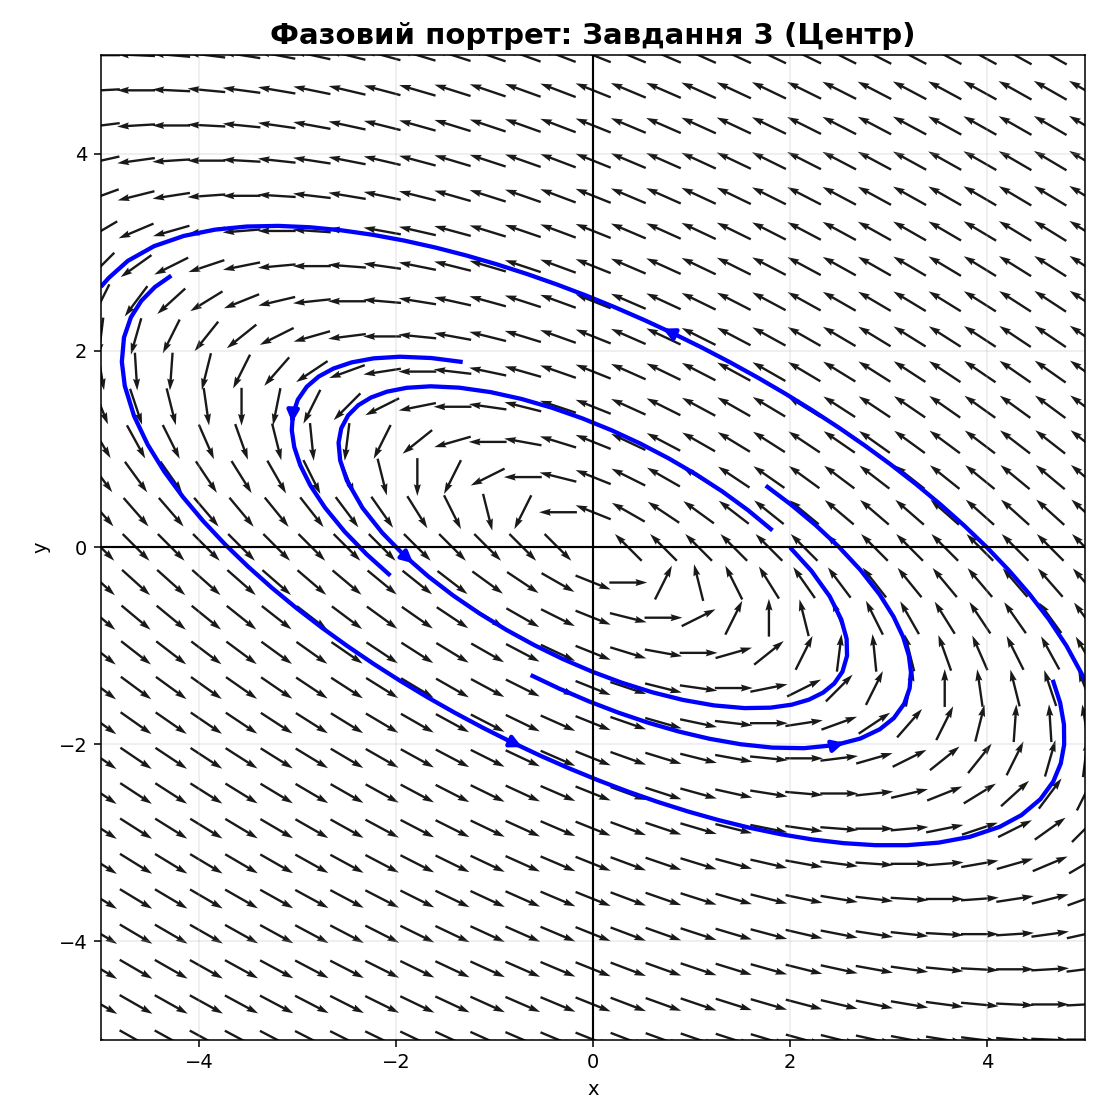
\includegraphics[width=0.85\textwidth]{portrait3_python.png}
    \caption{Фазовий портрет (Python) для Завдання 3}
\end{figure}

\subsection{Програмний розв'язок у Maple}
\begin{verbatim}
restart;
with(DEtools):
sys1 := {diff(x(t), t) = -2*x(t) - 5*y(t), diff(y(t), t) = 2*x(t) + 2*y(t)};

# Analytic solution
sol1 := dsolve(sys1);
print("Analytic solution:", sol1);

# Phase portrait
DEplot(sys1, [x(t), y(t)], t = -10 .. 10, x = -5 .. 5, y = -5 .. 5,
       [[x(0)=2, y(0)=0], [x(0)=4, y(0)=0]],
       arrows = MEDIUM, stepsize = 0.05,
       title = "Phase portrait: Center", color = black, linecolor = blue);
\end{verbatim}

\begin{figure}[H]
    \centering
    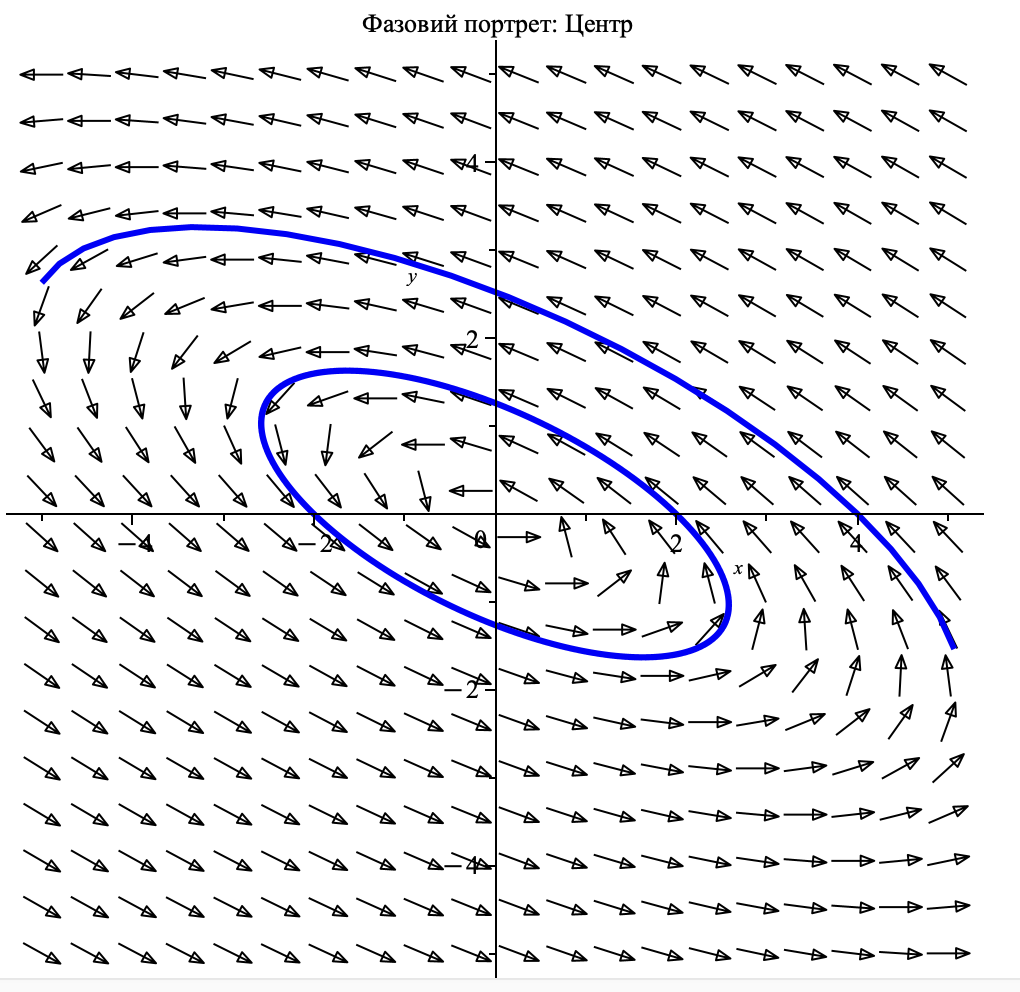
\includegraphics[width=0.85\textwidth]{portrait_1.png}
    \caption{Фазовий портрет для Завдання 3 (центр)}
\end{figure}

\begin{figure}[H]
    \centering
    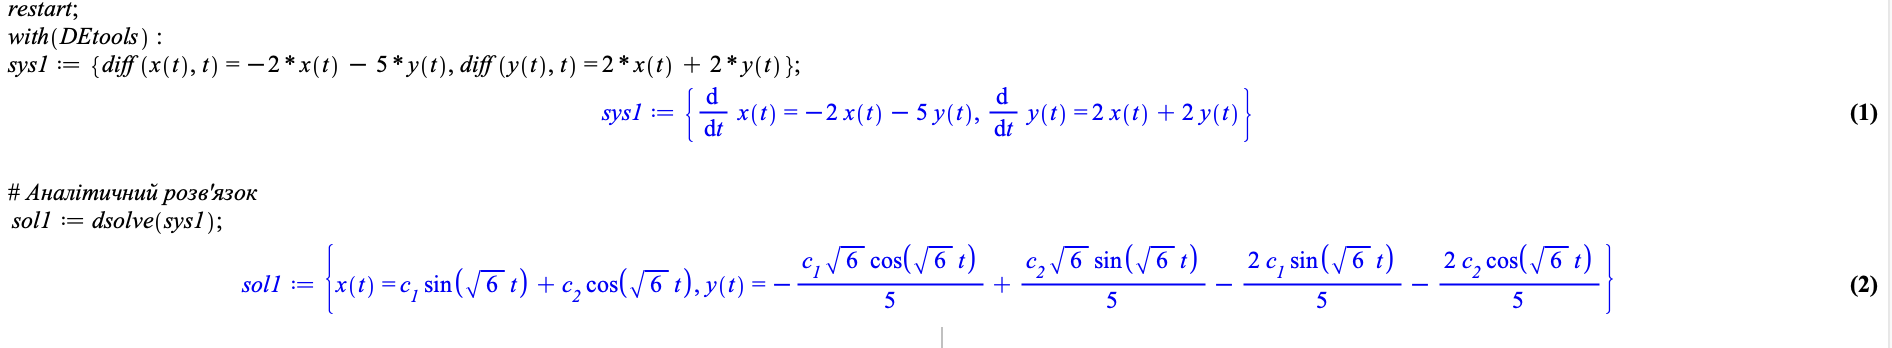
\includegraphics[width=0.78\textwidth]{solve3.png}
    \caption{Скріншот аналітичного розв'язку у Maple для Завдання 3}
\end{figure}

\section{Завдання 6}

\subsection{Запис системи та матриці}

Розглянемо лінійну стаціонарну систему на площині:
\[
\begin{cases}
\dot{x} = x, \\
\dot{y} = 2x - y.
\end{cases}
\]
Матриця системи має вигляд
\[
A =
\begin{pmatrix}
1 & 0\\
2 & -1
\end{pmatrix}.
\]

\subsection{Характеристичне рівняння та класифікація особливої точки}

Складемо характеристичне рівняння $\det(A - \lambda I) = 0$:
\[
\begin{vmatrix}
1-\lambda & 0\\
2 & -1-\lambda
\end{vmatrix}
= (1-\lambda)(-1-\lambda) - 0
= -(1-\lambda)(1+\lambda)
= \lambda^2 - 1 = 0.
\]
Звідси власні числа матриці:
\[
\lambda_1 = 1, \qquad \lambda_2 = -1.
\]
Власні значення дійсні та мають різні знаки ($\lambda_1 > 0$, $\lambda_2 < 0$). Отже, положення рівноваги $(0,0)$ є \textbf{сідлом}. Ця особлива точка є нестійкою.

\subsection{Побудова перетвореної системи}

\subsubsection{Власні вектори та заміна координат}

Знайдемо власний вектор для $\lambda_1 = 1$. Розв'яжемо $(A - I)\,v = 0$:
\[
\begin{pmatrix}
0 & 0\\
2 & -2
\end{pmatrix}
\begin{pmatrix}
v_1\\v_2
\end{pmatrix}
=
\begin{pmatrix}
0\\0
\end{pmatrix}.
\]
З другого рядка: $2v_1 - 2v_2 = 0$, тобто $v_1 = v_2$. Покладемо $v_2 = 1$:
\[
V_1 =
\begin{pmatrix}
1\\1
\end{pmatrix}.
\]

Знайдемо власний вектор для $\lambda_2 = -1$. Розв'яжемо $(A + I)\,v = 0$:
\[
\begin{pmatrix}
2 & 0\\
2 & 0
\end{pmatrix}
\begin{pmatrix}
v_1\\v_2
\end{pmatrix}
=
\begin{pmatrix}
0\\0
\end{pmatrix}.
\]
Звідси $v_1 = 0$, а $v_2$~--- довільне. Покладемо $v_2 = 1$:
\[
V_2 =
\begin{pmatrix}
0\\1
\end{pmatrix}.
\]

Запишемо лінійне неособливе перетворення, стовпцями якого є власні вектори:
\[
\begin{pmatrix}
x\\y
\end{pmatrix}
=
\begin{pmatrix}
1 & 0\\
1 & 1
\end{pmatrix}
\begin{pmatrix}
\xi\\\eta
\end{pmatrix},
\]
тобто
\[
x = \xi, \qquad y = \xi + \eta.
\]
Обернене перетворення:
\[
\xi = x, \qquad \eta = y - x.
\]

\subsubsection{Виведення перетвореної системи}

Покажемо, що в координатах $(\xi,\eta)$ система набуває діагонального вигляду.

Оскільки $\xi = x$, маємо
\[
\dot{\xi} = \dot{x} = x = \xi.
\]

Далі, $\eta = y - x$, тому
\[
\dot{\eta} = \dot{y} - \dot{x} = (2x - y) - x = x - y.
\]
Виразимо через нові змінні: $x - y = \xi - (\xi + \eta) = -\eta$, отже
\[
\dot{\eta} = -\eta.
\]

Таким чином, перетворена система має вигляд
\[
\dot{\xi} = \xi, \qquad \dot{\eta} = -\eta,
\]
що є канонічною діагональною формою для сідла.

\subsection{Загальний розв'язок перетвореної системи та сепаратриси}

Кожне з рівнянь перетвореної системи розв'язується незалежно:
\[
\xi(t) = C_1\,e^t, \qquad \eta(t) = C_2\,e^{-t}.
\]
Виключаючи час, отримуємо рівняння фазових траєкторій у площині $(\xi,\eta)$:
\[
\xi\,\eta = C_1\,C_2 = \mathrm{const}.
\]
Це сім'я гіпербол із осями $\xi$ і $\eta$ як асимптотами.

\begin{figure}[H]
    \centering
    
\includegraphics[width=0.72\textwidth]{hyperbolas_xi_eta.png}
    \caption{Гіперболи $\xi\,\eta=C$ у перетвореній системі $(\xi,\eta)$ для Завдання~6}
\end{figure}

\textbf{Сепаратриси} перетвореної системи:
\begin{itemize}
    \item $\eta = 0$ ($C_2 = 0$): траєкторія $\xi(t) = C_1\,e^t$, рух від початку координат при $t \to +\infty$;
    \item $\xi = 0$ ($C_1 = 0$): траєкторія $\eta(t) = C_2\,e^{-t}$, рух до початку координат при $t \to +\infty$.
\end{itemize}

\subsection{Фазовий портрет у початкових координатах}

Після оберненого перетворення $\xi = x$, $\eta = y - x$ сепаратриси набувають вигляду:
\begin{itemize}
    \item $\eta = 0 \;\Leftrightarrow\; y = x$~--- нестійка сепаратриса (траєкторії віддаляються від початку координат вздовж прямої $y = x$, оскільки $\lambda_1 = 1 > 0$);
    \item $\xi = 0 \;\Leftrightarrow\; x = 0$~--- стійка сепаратриса (траєкторії наближаються до початку координат вздовж осі $y$, оскільки $\lambda_2 = -1 < 0$).
\end{itemize}

Інші фазові траєкторії мають гіперболічний характер: при $t \to +\infty$ вони наближаються до нестійкої сепаратриси $y = x$, а при $t \to -\infty$~--- до стійкої сепаратриси $x = 0$.

Рівняння сім'ї траєкторій у початкових координатах отримуємо з $\xi\,\eta = \mathrm{const}$:
\[
x\,(y - x) = \mathrm{const}.
\]

\begin{figure}[H]
    \centering
    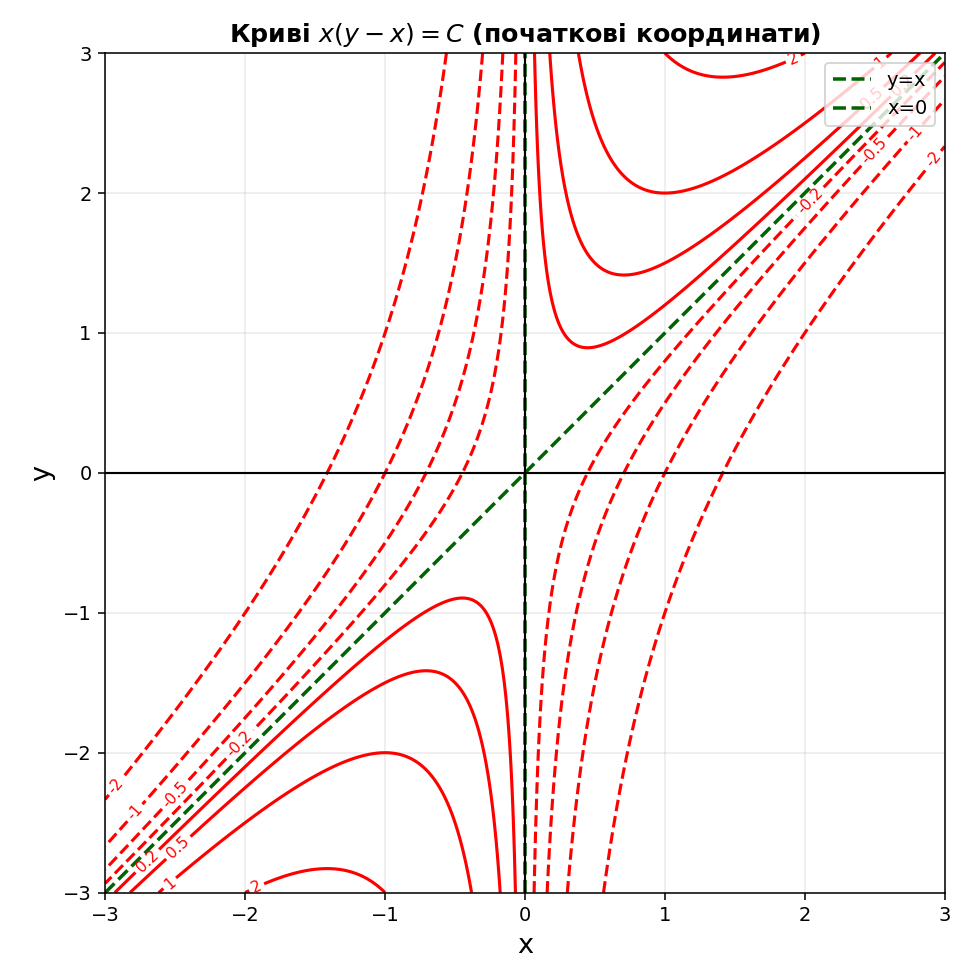
\includegraphics[width=0.72\textwidth]{saddle_curves_xy.png}
    \caption{Криві $x(y-x)=C$ та сепаратриси у початкових координатах для Завдання~6}
\end{figure}

\subsection{Аналітичний розв'язок системи}

Побудуємо загальний розв'язок зведенням до рівняння другого порядку. З першого рівняння $\dot{x} = x$ одразу маємо
\[
x(t) = C_1\,e^t.
\]
Підставимо у друге рівняння $\dot{y} = 2x - y$:
\[
\dot{y} + y = 2C_1\,e^t.
\]
Це лінійне неоднорідне рівняння першого порядку. Його однорідний розв'язок: $y_{\text{одн}} = C_2\,e^{-t}$. Частинний розв'язок шукаємо у вигляді $y_{\text{ч}} = B\,e^t$. Підставляючи:
\[
B\,e^t + B\,e^t = 2C_1\,e^t \;\Rightarrow\; 2B = 2C_1 \;\Rightarrow\; B = C_1.
\]
Отже, загальний розв'язок:
\[
\begin{cases}
x(t) = C_1\,e^t,\\
y(t) = C_1\,e^t + C_2\,e^{-t}.
\end{cases}
\]

\subsection{Висновок до Завдання 6}

Характеристичне рівняння системи має дійсні корені різних знаків $\lambda_1 = 1$, $\lambda_2 = -1$. Особлива точка $(0,0)$ є сідлом. Після лінійного неособливого перетворення система зводиться до діагональної форми, у якій фазові траєкторії є гіперболами. У початкових координатах сепаратрисами є прямі $y = x$ (нестійка) та $x = 0$ (стійка), а решта траєкторій описується рівнянням $x(y-x) = \mathrm{const}$.

\begin{figure}[H]
    \centering
    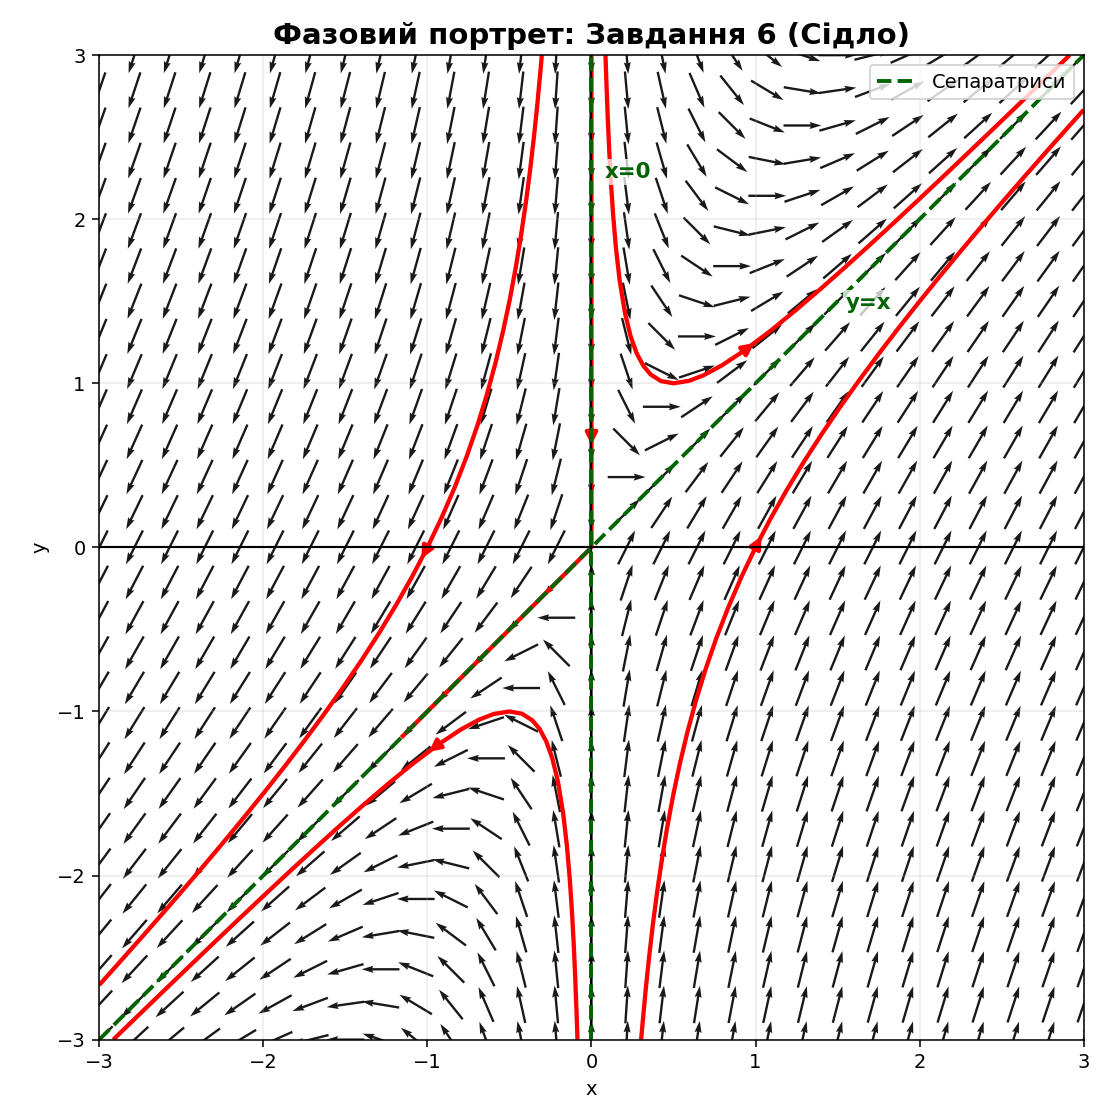
\includegraphics[width=0.85\textwidth]{portrait6_python.png}
    \caption{Фазовий портрет (Python) для Завдання 6}
\end{figure}

\subsection{Програмний розв'язок у Maple}
\begin{verbatim}
restart;
with(DEtools):
sys2 := {diff(x(t), t) = x(t), diff(y(t), t) = 2*x(t) - y(t)};

# Analytic solution
sol2 := dsolve(sys2);
print("Analytic solution:", sol2);

# Phase portrait
DEplot(sys2, [x(t), y(t)], t = -5 .. 5, x = -3 .. 3, y = -3 .. 3,
       [[x(0)=1, y(0)=0], [x(0)=-1, y(0)=0],
        [x(0)=0.5, y(0)=1], [x(0)=-0.5, y(0)=-1]],
       arrows = MEDIUM, stepsize = 0.05,
       title = "Phase portrait: Saddle", color = black, linecolor = red);
\end{verbatim}

\begin{figure}[H]
    \centering
    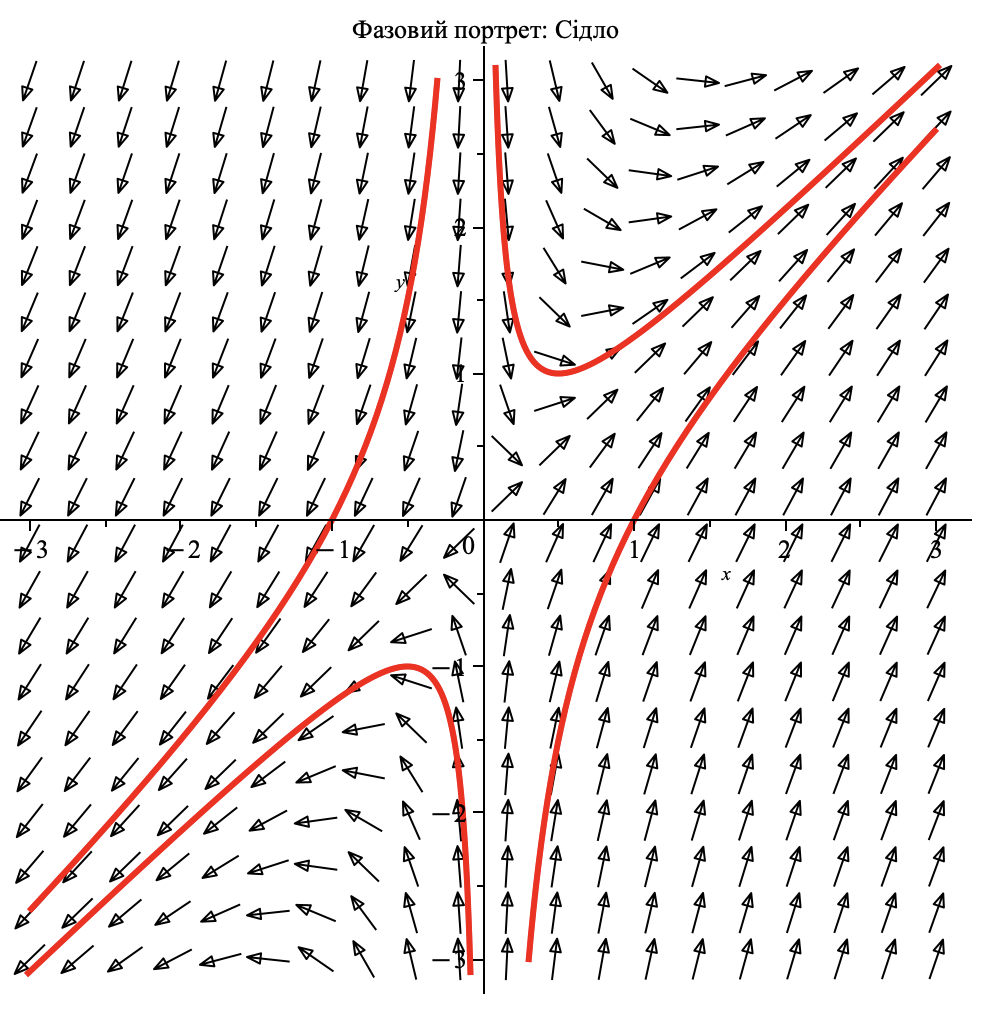
\includegraphics[width=0.85\textwidth]{portrait_2.png}
    \caption{Фазовий портрет для Завдання 6 (сідло)}
\end{figure}

\begin{figure}[H]
    \centering
    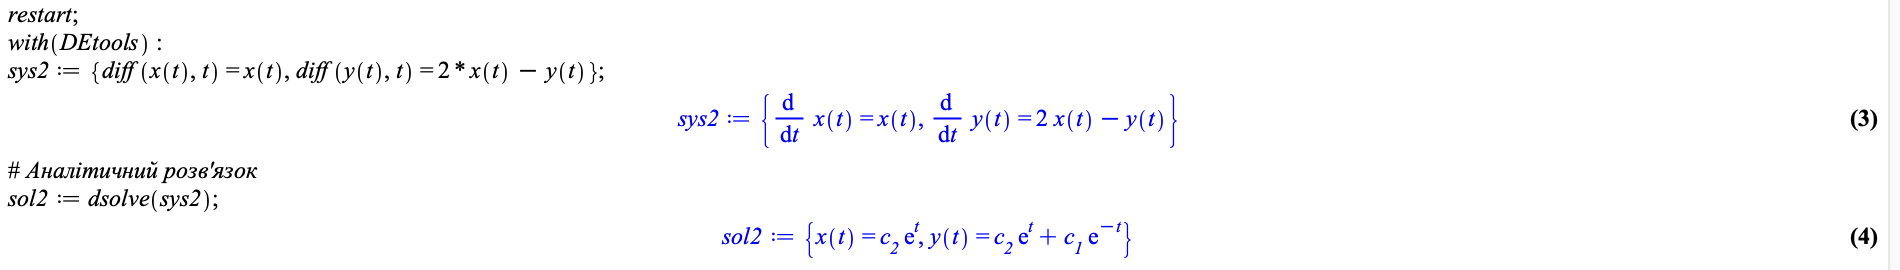
\includegraphics[width=0.78\textwidth]{solve6.png}
    \caption{Скріншот аналітичного розв'язку у Maple для Завдання 6}
\end{figure}

\end{document}
